\documentclass{beamer}
\usetheme{Warsaw}

\usepackage{enumerate}

\setbeamertemplate{footline}
{
  \leavevmode
  \hbox{
    \begin{beamercolorbox}[wd=.4\paperwidth,ht=2.25ex,dp=1ex,center]{author in head/foot}
        \usebeamerfont{whitespace}
    \end{beamercolorbox}
    \begin{beamercolorbox}[wd=.2\paperwidth,ht=2.25ex,dp=1ex,center]{title in head/foot}
        \hspace*{1em}
        \insertframenumber{}
        \hspace*{1em}
    \end{beamercolorbox}
    \begin{beamercolorbox}[wd=.4\paperwidth,ht=2.25ex,dp=1ex,center]{author in head/foot}
        \usebeamerfont{whitespace}
    \end{beamercolorbox}
  }
}

\makeatletter
\setbeamertemplate{navigation symbols}{}

\title[Or how my wife learnt about my ability to wreck a home network]{Homelab Escapades}
\subtitle{Newcastle Cybersecurity Group}
\author[Jay Rovacsek]{Jay Rovacsek}
\date{\today}

\begin{document}

\begin{frame}
\maketitle
\end{frame}

\section{Introduction}
\subsection{\$whoami}

\begin{frame}
    \begin{center}
        Public speaking skills: a solid 2.5/10 - remind me now that I should slow down and chill-out
    \end{center}
\end{frame}

\begin{frame}
    \begin{columns}
        \begin{column}{0.5\textwidth}
            If you have questions at any point feel free to jump in! 
        \end{column}
        \begin{column}{0.5\textwidth}
            \begin{figure}
                \centering
                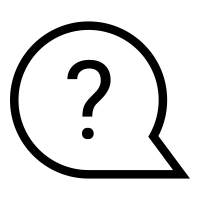
\includegraphics[width=\textwidth,keepaspectratio]{../resources/question.png}
            \end{figure}
        \end{column}
    \end{columns}
\end{frame}

\begin{frame}
    \begin{columns}
        \begin{column}{0.5\textwidth}
            \$whoami: I work for nib as part of the cybersecurity function
        \end{column}
        \begin{column}{0.5\textwidth}
            \begin{figure}
                \centering
                
\includegraphics[width=\textwidth,keepaspectratio]{../resources/smile.jpg}
            \end{figure}
        \end{column}
    \end{columns}
\end{frame}

\begin{frame}
    \begin{columns}
        \begin{column}{0.5\textwidth}
            Previous lives as: 
            \begin{itemize}
                \item developer
                \item retail assistant
                \item pizza cutter
                \item lawn mower
            \end{itemize}
        \end{column}
        \begin{column}{0.5\textwidth}
            \begin{figure}
                \centering
                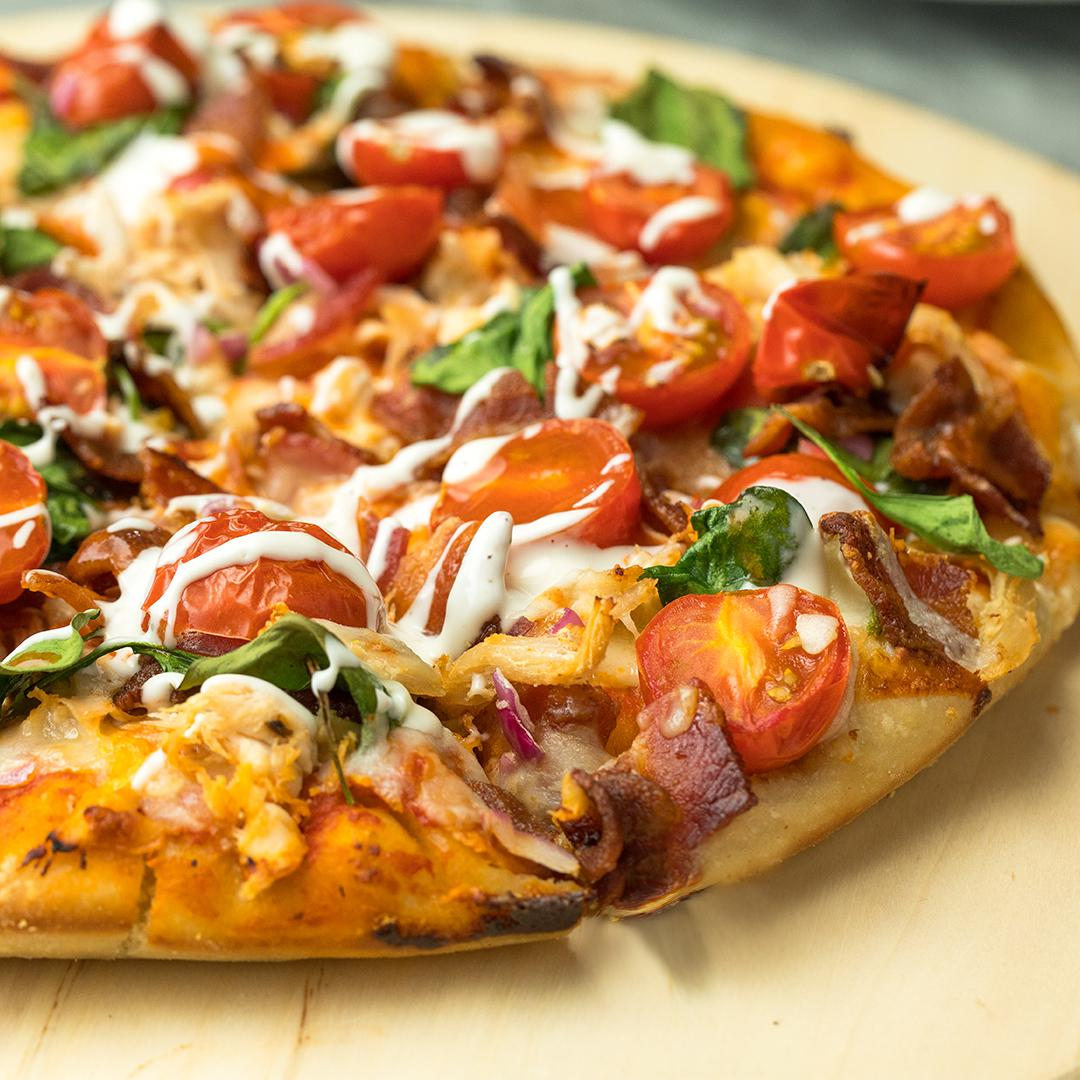
\includegraphics[width=\textwidth,keepaspectratio]{../resources/pizza.jpg}
            \end{figure}
        \end{column}
    \end{columns}
\end{frame}

\begin{frame}
    \begin{columns}
        \begin{column}{0.5\textwidth}
            What am I not? 
            \begin{itemize}
                \item A sysadmin
                \item Good at making presentation slides
            \end{itemize}
        \end{column}
        \begin{column}{0.5\textwidth}
            \begin{figure}
                \centering
                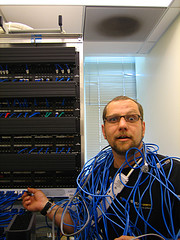
\includegraphics[width=\textwidth,keepaspectratio]{../resources/sysadmin.jpg}
            \end{figure}
        \end{column}
    \end{columns}
\end{frame}

\begin{frame}
    \begin{columns}
        \begin{column}{0.5\textwidth}
            Does any of this matter?
            \vspace{5mm}\par\noindent
            Just keep in mind, I'm just some dude throwing some things together
            and hoping for the best
        \end{column}
        \begin{column}{0.5\textwidth}
            \begin{figure}
                \centering
                
\includegraphics[width=\textwidth,keepaspectratio]{../resources/nope.jpg}
            \end{figure}
        \end{column}
    \end{columns}
\end{frame}

\subsection{Home Networks eh?}

\begin{frame}
    \begin{columns}
        \begin{column}{0.5\textwidth}
            But why am I here presenting?
        \end{column}
        \begin{column}{0.5\textwidth}
            \begin{figure}
                \centering
                
\includegraphics[width=\textwidth,keepaspectratio]{../resources/shrug.jpg}
            \end{figure}
        \end{column}
    \end{columns}
\end{frame}

\begin{frame}
    \begin{itemize}
        \item Home networks are fun
        \item Breaking your own stuff will assist in teaching you
        \item Can run some cool services for yourself/family/friends
    \end{itemize}
\end{frame}

\begin{frame}
    \begin{center}
        I originally started writing this presentation deck in a manner that 
        I reflected on and felt it was going to be telling some of the audience to 
        suck eggs.
    \end{center}
\end{frame}

\begin{frame}
    \begin{center}
        Instead at the end of these slides we'll open to discussion on the content and 
        have a look at some of the home network protections I've setup
    \end{center}
\end{frame}

\begin{frame}
    \begin{center}
        I totally won't regret this.
    \end{center}
\end{frame}

\begin{frame}
    \begin{center}
        Who is currently running their own hobby networks?
        \vspace{5mm}\par\noindent
        What are you currently running?
    \end{center}
\end{frame}

\begin{frame}
    \begin{columns}
        \begin{column}{0.5\textwidth}
            Are there reasons to not run a service on your home network?
        \end{column}
        \begin{column}{0.5\textwidth}
            \begin{figure}
                \centering
                
\includegraphics[width=\textwidth,keepaspectratio]{../resources/confusion.jpg}
            \end{figure}
        \end{column}
    \end{columns}
\end{frame}

\begin{frame}
    \begin{center}
        What might we do to a home network to not secure it?
    \end{center}
\end{frame}

\begin{frame}
    \begin{itemize}
        \item Disparate, inconsistent, or no authentication on services
        \item Failure to segment devices based on use-case or trust of the devices
        \item Not implement any basic IPS/IDS
        \item Not ensure egress traffic utilising insecure protocols are managed suitably (DNSSEC, DoH or DoTLS enforcement)
        \item No analysis of traffic patterns
    \end{itemize}
\end{frame}

\section{Building A Home Network}
\subsection{What Might We Run?}

\begin{frame}
    \begin{columns}
        \begin{column}{0.5\textwidth}
            What services might we want to run?
        \end{column}
        \begin{column}{0.5\textwidth}
            \begin{figure}
                \centering
                
\includegraphics[width=\textwidth,keepaspectratio]{../resources/logos.png}
            \end{figure}
        \end{column}
    \end{columns}
\end{frame}

\begin{frame}
    \begin{columns}
        \begin{column}{0.5\textwidth}
            Should we expose these services?
        \end{column}
        \begin{column}{0.5\textwidth}
            \begin{figure}
                \centering
                
\includegraphics[width=\textwidth,keepaspectratio]{../resources/logos.png}
            \end{figure}
        \end{column}
    \end{columns}
\end{frame}

\subsection{Moar Access, Moar Problems}

\begin{frame}
    \begin{columns}
        \begin{column}{0.5\textwidth}
            I want to be able to access my services from anywhere!
        \end{column}
        \begin{column}{0.5\textwidth}
            \begin{figure}
                \centering
                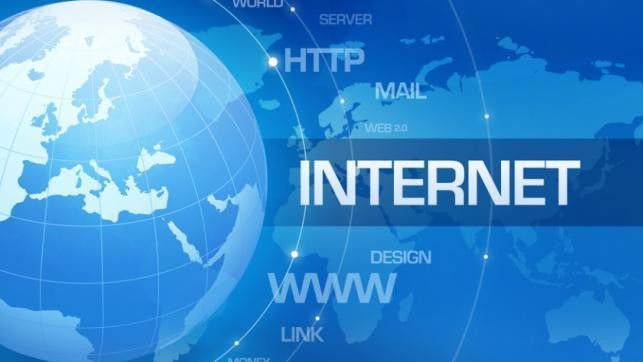
\includegraphics[width=\textwidth]{../resources/internet.jpg}
            \end{figure}
        \end{column}
    \end{columns}
\end{frame}

\begin{frame}
    \begin{center}
        Cheatsheet for building a home network:
    \end{center}
    \begin{enumerate}
        \item Buy a domain, or use a freebie
        \item Pester your ISP for a static address (or big-brain it with some dynamic DNS)
        \item Setup some port forwards
        \item ????
        \item Profit!
    \end{enumerate}
\end{frame}


\begin{frame}
    \begin{center}
        \textit{fin}
    \end{center}
\end{frame}

\begin{frame}
    \begin{center}
        Okay, cool, I have the things available on the interwebs...
    \end{center}
\end{frame}


\begin{frame}
    \begin{columns}
        \begin{column}{0.5\textwidth}
            Should we leaving our applications in a default state?
        \end{column}
        \begin{column}{0.5\textwidth}
            \begin{figure}
                \centering
                
\includegraphics[width=\textwidth,keepaspectratio]{../resources/oprah.png}
            \end{figure}
        \end{column}
    \end{columns}
\end{frame}

\subsection{Could We Secure Exposed Services Better?}

\begin{frame}
    \begin{columns}
        \begin{column}{0.5\textwidth}
            Nope! Let's apply some defence in depth!
        \end{column}
        \begin{column}{0.5\textwidth}
            \begin{figure}
                \centering
                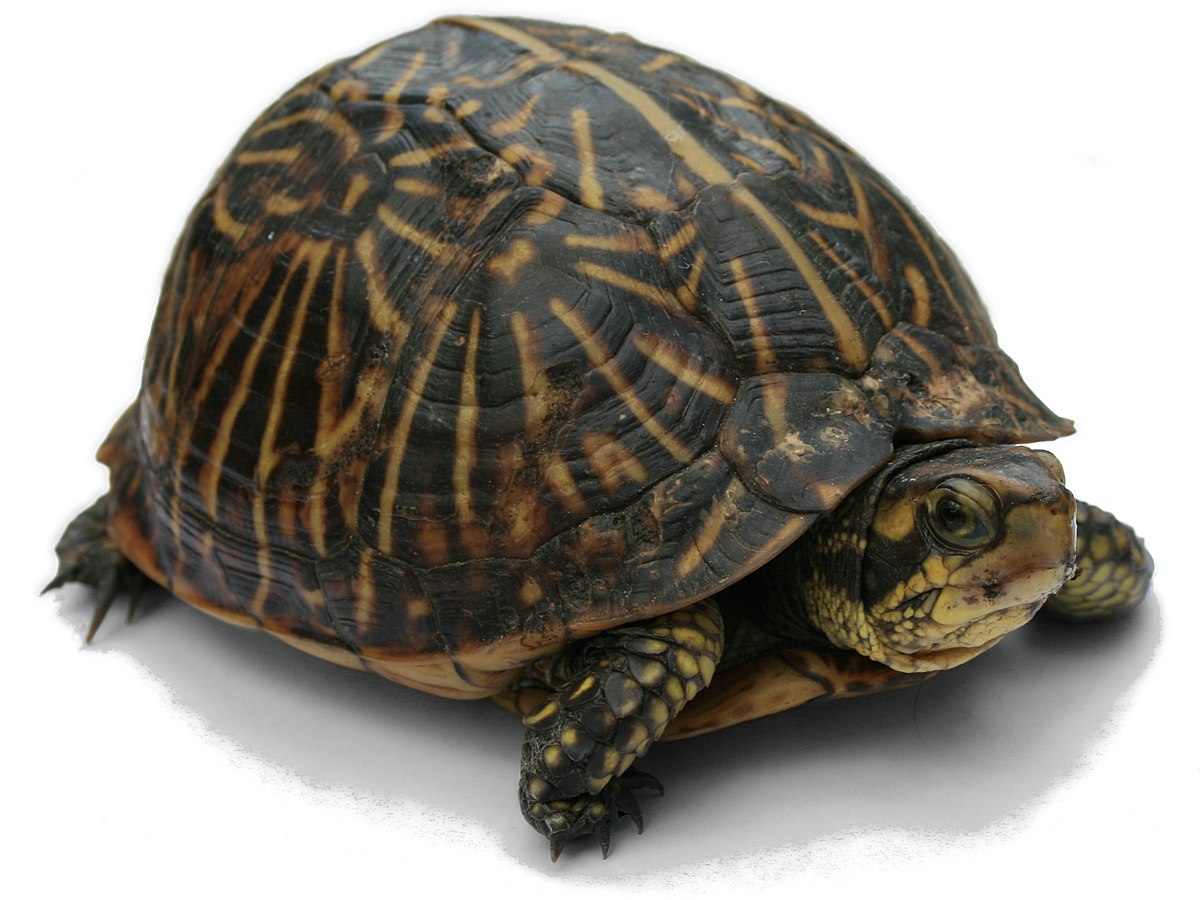
\includegraphics[width=\textwidth,keepaspectratio]{../resources/turtle.jpg}
            \end{figure}
        \end{column}
    \end{columns}
\end{frame}

\begin{frame}
    I happen to have killed hours of my spare time implementing:
    \begin{itemize}
        \item Overkill network segmentation (sorry Sarah, I'll fix your chromecast connectivity one day)
        \item Traffic analysis via Snort
        \item Transparent DNS request rewrites via a DoH proxy
        \item Consistent authentication for my exposed services (there are limits here)
    \end{itemize}
    I am still looking to kill hours of my time with:
    \begin{itemize}
        \item Analysis of traffic patterns to identify potential issues (Zeek)
    \end{itemize}
\end{frame}

\begin{frame}
    Is anyone currently utilising Zeek or have any insight into traffic pattern analysis?
\end{frame}

\begin{frame}
    Let's talk about free options that preserve privacy and security while imposing 
    very little technical barrier to entry:
    \begin{itemize}
        \item Authelia (strong authentication protections on all yo' things)
        \item Pfsense/OPSense (or why you shouldn't accept your ISPs garbage)
        \item Snort (proactive blocking of script kiddies)
    \end{itemize}
\end{frame}

\begin{frame}
    If we have time at the end of this talk I'd love to talk about some items that are
    less about homelab security and more about individual security:
    \begin{itemize}
        \item Approaches to backups
        \item Self management of secrets (getting out of the potential trap that is SaaS Password Managers)
        \item Implementing your own VPN (should you?)
    \end{itemize}
\end{frame}

\begin{frame}
    \begin{columns}
        \begin{column}{0.5\textwidth}
            Ever looked at the dumpsterfire that is an nginx config?
        \end{column}
        \begin{column}{0.5\textwidth}
            \begin{figure}
                \centering
                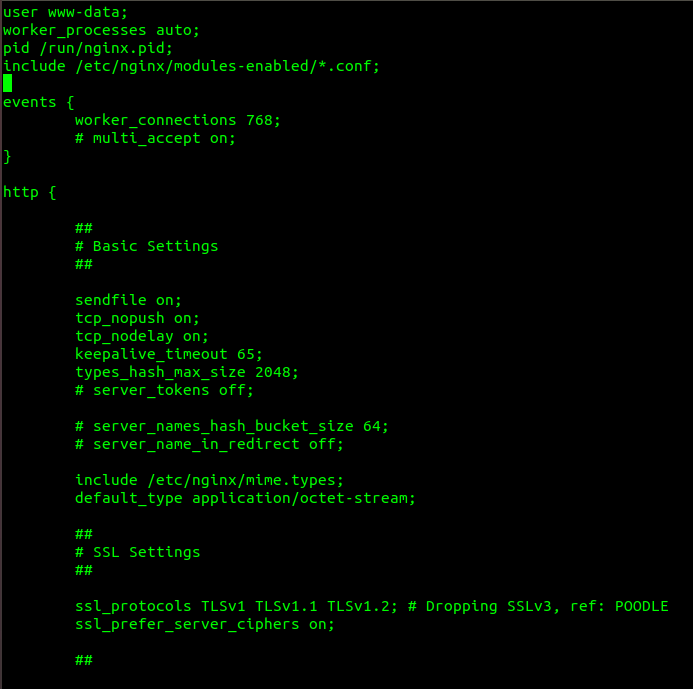
\includegraphics[width=\textwidth,keepaspectratio]{../resources/nginx_config.png}
            \end{figure}
        \end{column}
    \end{columns}
\end{frame}

\begin{frame}
    \begin{columns}
        \begin{column}{0.5\textwidth}
            I don't actually mind them, but we'll assume that we ain't got time for that
        \end{column}
        \begin{column}{0.5\textwidth}
            \begin{figure}
                \centering
                
\includegraphics[width=\textwidth,keepaspectratio]{../resources/nobody_got_time.jpg}
            \end{figure}
        \end{column}
    \end{columns}
\end{frame}

\begin{frame}
    \begin{columns}
        \begin{column}{0.3\textwidth}
            Get some SWAG!
        \end{column}
        \begin{column}{0.7\textwidth}
            \begin{figure}
                \centering
                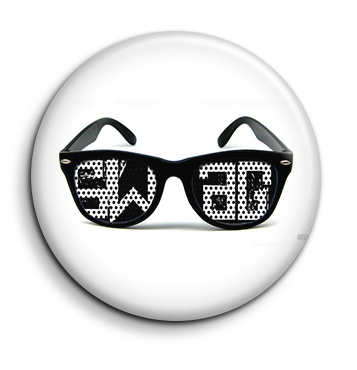
\includegraphics[width=\textwidth,keepaspectratio]{../resources/wrong_swag.jpg}
            \end{figure}
        \end{column}
    \end{columns}
\end{frame}


\begin{frame}
    \begin{figure}
        \centering
        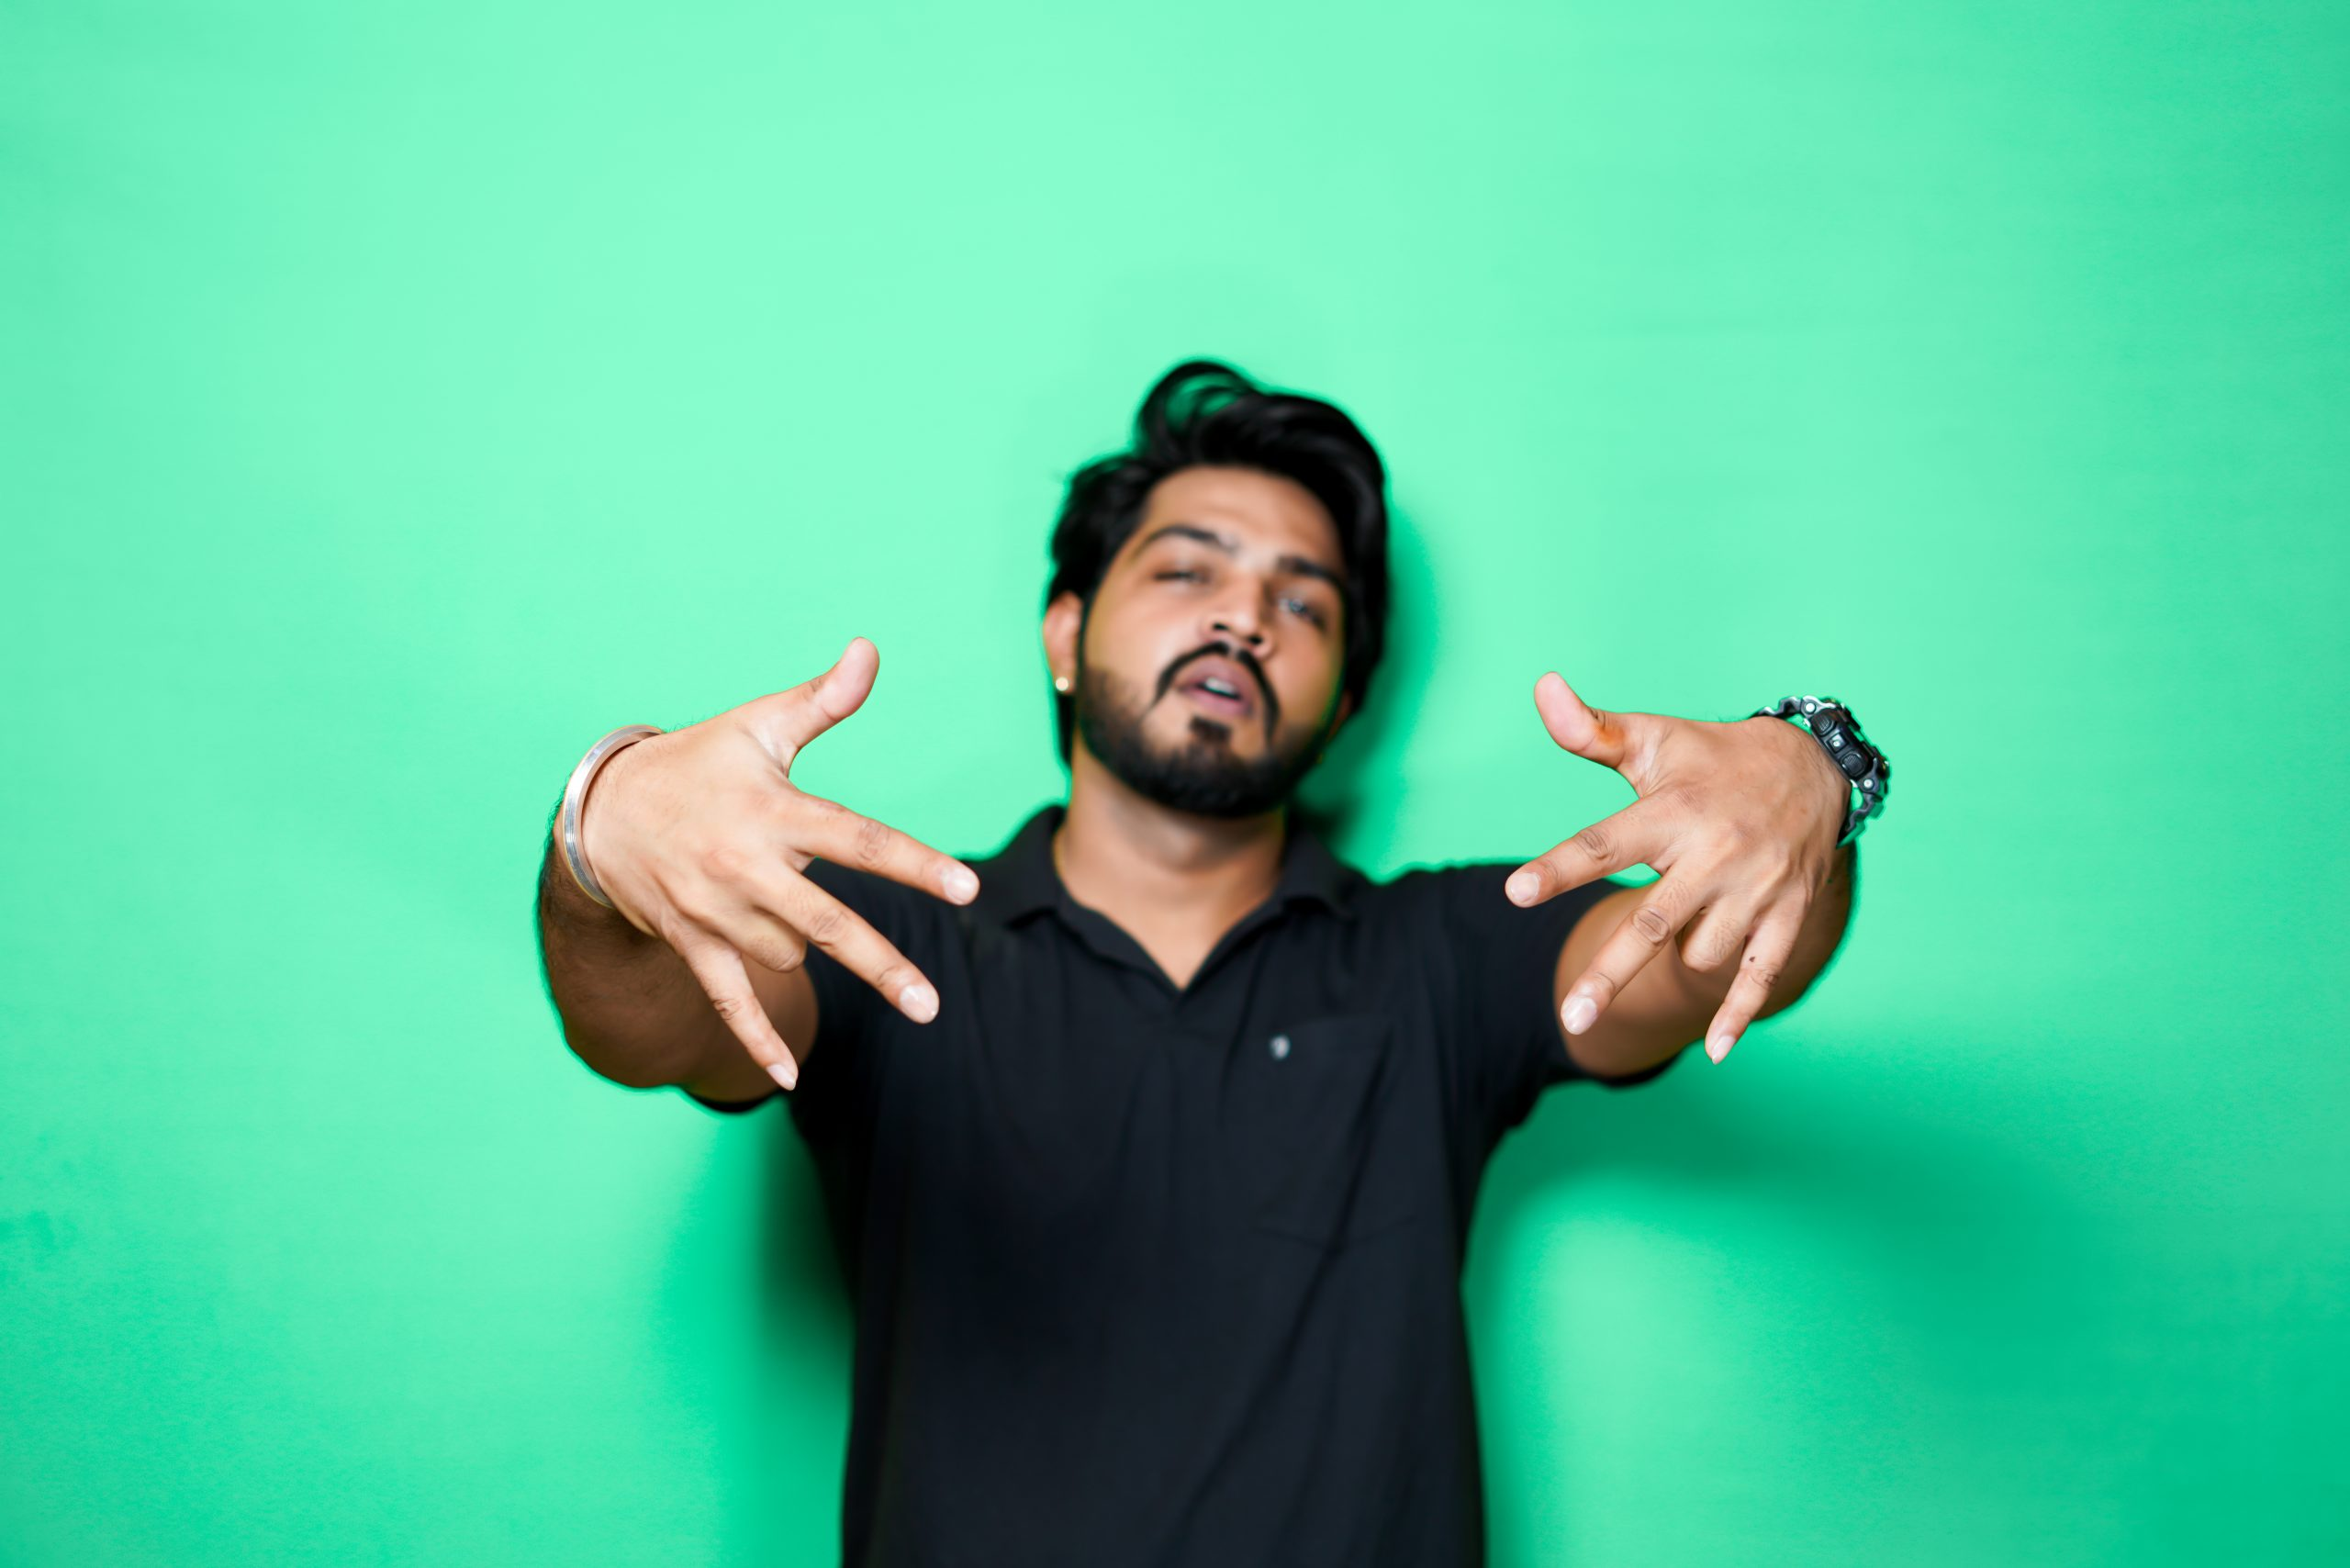
\includegraphics[width=\textwidth,keepaspectratio]{../resources/wrong_swag2.jpg}
    \end{figure}
\end{frame}

\begin{frame}
    \begin{figure}
        \centering
        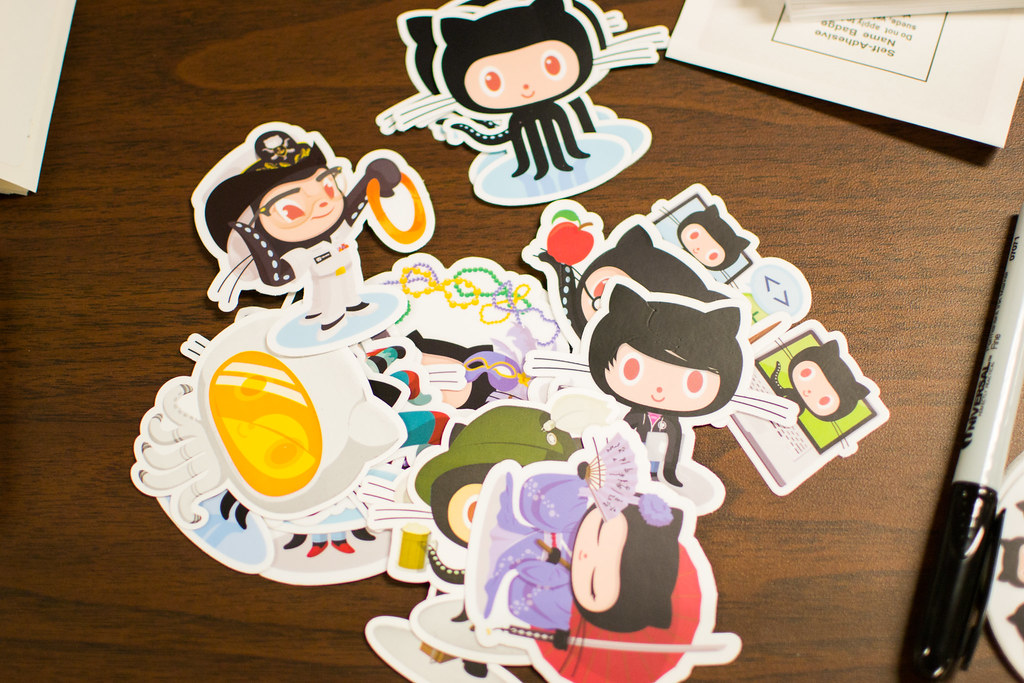
\includegraphics[width=\textwidth,keepaspectratio]{../resources/wrong_swag3.jpg}
    \end{figure}
\end{frame}

\begin{frame}
    \begin{columns}
        \begin{column}{0.7\textwidth}
            This SWAG... \href{https://github.com/linuxserver/docker-swag}{https://github.com/linuxserver/docker-swag}
        \end{column}
        \begin{column}{0.3\textwidth}
            \begin{figure}
                \centering
                
\includegraphics[width=\textwidth,keepaspectratio]{../resources/swag.png}
            \end{figure}
        \end{column}
    \end{columns}
\end{frame}

\section{Authelia}
\subsection{SWAG}

\begin{frame}
    \begin{center}
        Why SWAG?
    \end{center}
    \begin{itemize}
        \item It's a batteries included approach to us getting Authelia in the mix.
        \item It contains default configs for nginx come with options for Authelia included but disabled.
        \item Includes Let's Encrypt automation in the box 
    \end{itemize}
\end{frame}

\begin{frame}
    \begin{center}
        Note: \textbf{SWAG is not required, it will just make your life easier in managing your reverse proxy \& Authelia}
        \vspace{5mm}\par\noindent
        If you have the know-how of setting up a reverse proxy of your choosing, you could do so. 
        \vspace{5mm}\par\noindent
        You could use HAProxy or Traefik instead if you're inclined
    \end{center}
\end{frame}

\subsection{Deployment Model}

\begin{frame}
    We're looking to deploy this model to our network:
    \begin{figure}
        \centering
        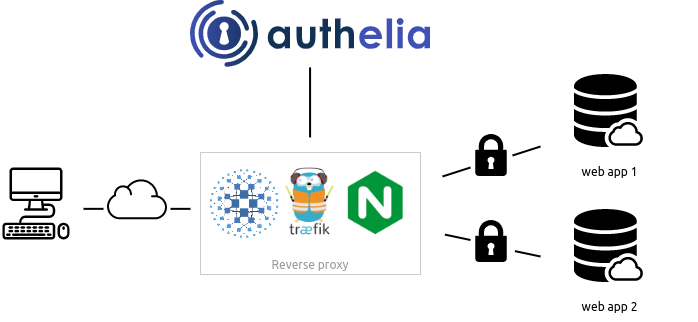
\includegraphics[width=\textwidth,keepaspectratio]{../resources/archi.png}
    \end{figure}
\end{frame}

\begin{frame}
    \begin{center}
        So we've got SWAG and Authelia setup, what does this achieve?    
    \end{center}
    \vspace{5mm}\par\noindent
    \begin{columns}
        \begin{column}{0.5\textwidth}
            \begin{figure}
                \centering
                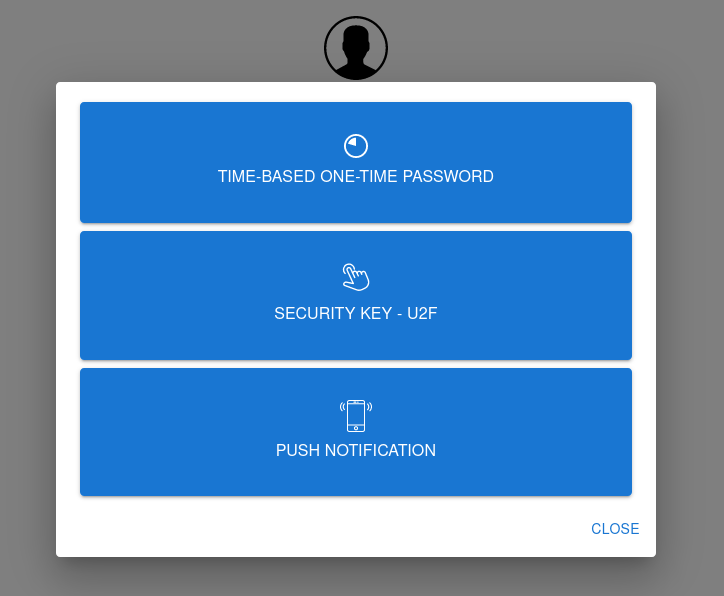
\includegraphics[width=\textwidth,keepaspectratio]{../resources/2fa_options.png}
            \end{figure}
        \end{column}
        \begin{column}{0.5\textwidth}
            \begin{figure}
                \centering
                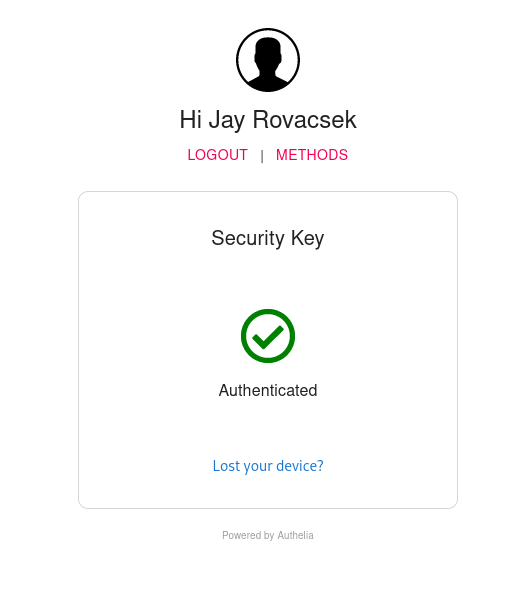
\includegraphics[width=\textwidth,keepaspectratio]{../resources/2fa_options_alt.png}
            \end{figure}
        \end{column}
    \end{columns}
\end{frame}

\begin{frame}
    \begin{center}
        Does this mean I could remove authentication from my exposed services?
        \vspace{5mm}\par\noindent
        Yup! (well, kinda)
        \vspace{5mm}\par\noindent
        
\includegraphics[height=0.5\textheight,keepaspectratio]{../resources/look_ma_no_auth.png}
    \end{center}
\end{frame}

\subsection{Live Demo?}

\begin{frame}
    \begin{center}
        What does the authentication flow look like? (do we chance a live demo?)
    \end{center}
\end{frame}

\begin{frame}
    \begin{center}
        Cool, that's pretty much Authelia
        \vspace{5mm}\par\noindent
        Any questions?
    \end{center}
\end{frame}

\begin{frame}
    \begin{center}
        Let's discuss home networks some more:
    \end{center}
    \begin{itemize}
        \item Open Source Firewalls
        \item IPS/IDS
        \item Backups
        \item Self management of secrets
        \item Implementing your own VPN
        \item Something else?
    \end{itemize}
\end{frame}


\end{document}